\begin{frame}{DAGuE}
\framesubtitle{Quick presentation}
\begin{center}
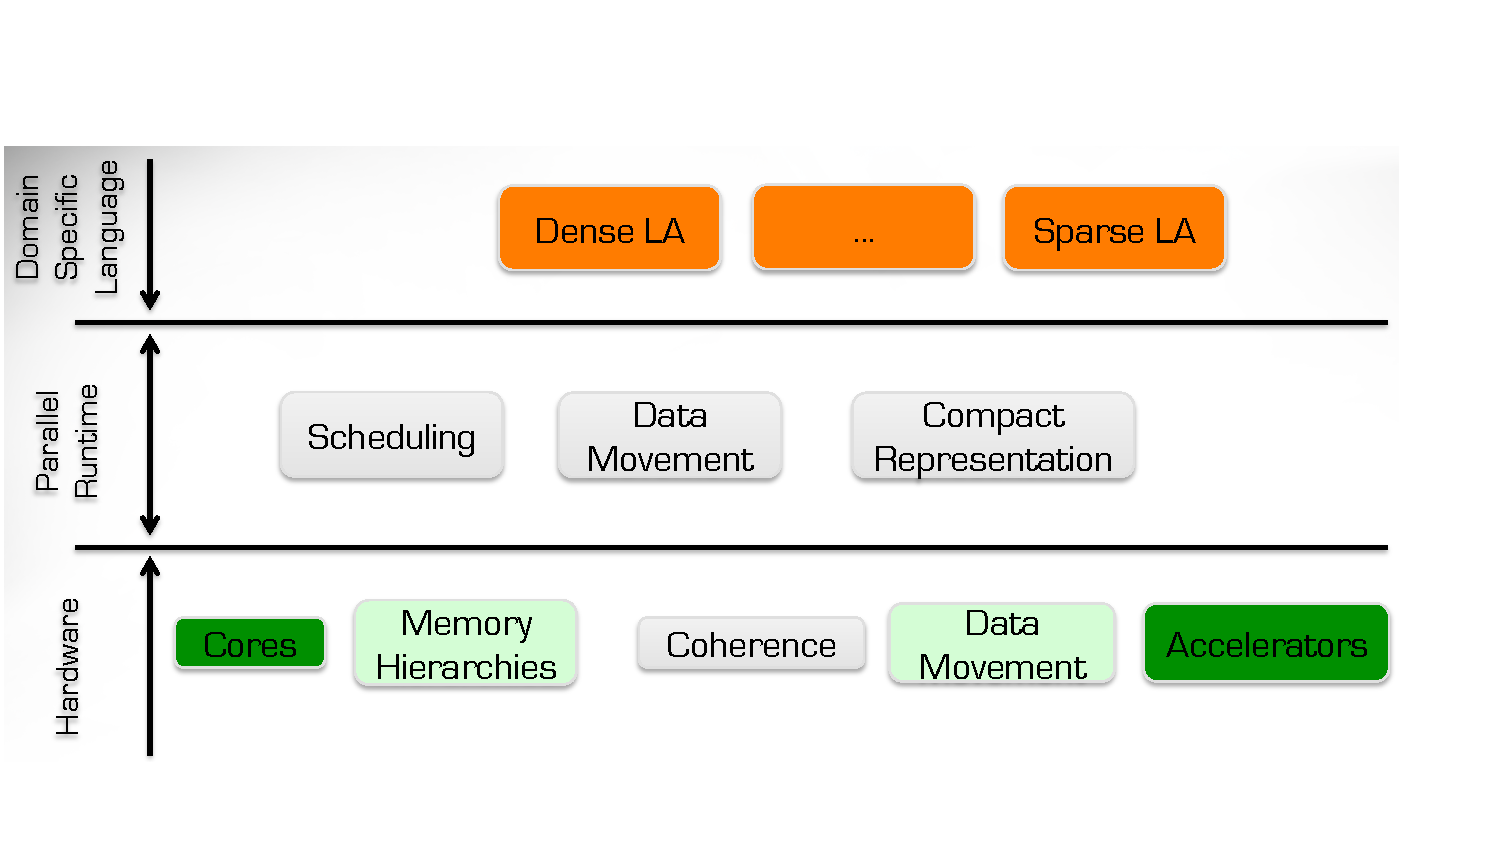
\includegraphics[scale=0.5]{3layer.pdf}
\end{center}
\end{frame}

\begin{frame}{DAGuE}
\framesubtitle{Quick presentation}
DAGuE is a Direct Acyclic Graph scheduler Engine based on task flow model where :
\begin{itemize}
\item nodes are tasks
\item edges are dependencies
\end{itemize}
\begin{center}
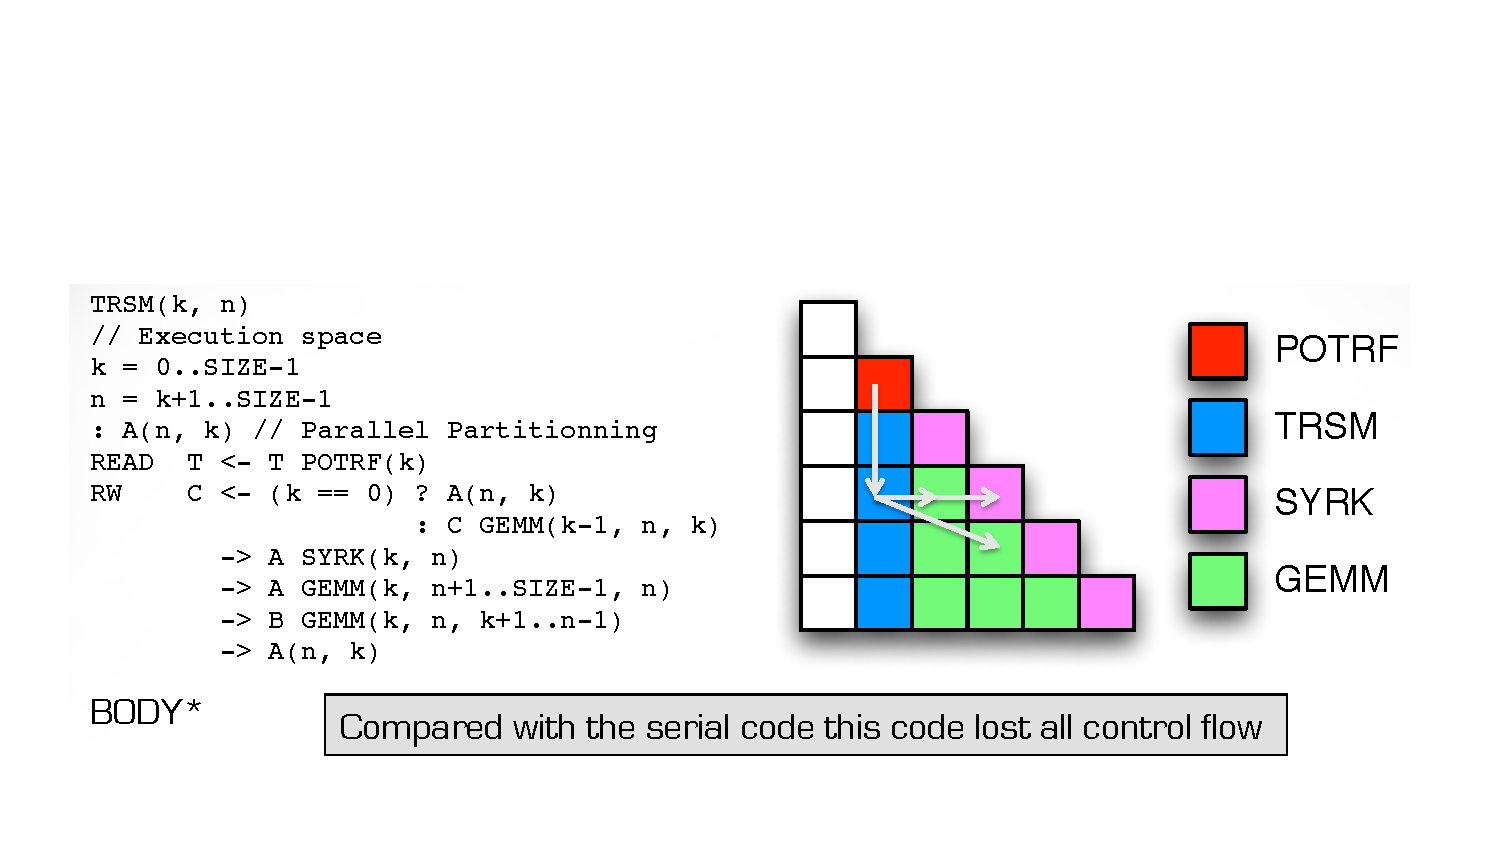
\includegraphics[scale=0.5]{trsm.pdf}
\end{center}
\end{frame}

\begin{frame}{DAGuE}
\begin{exampleblock}{Advantages :}
\begin{itemize}
\item Independence between performances and computers
\item Provide multicore parallelism
\item Good reactivity for load imbalance
\item Natural look ahead
\end{itemize}
\end{exampleblock}{}
\pause
\begin{exampleblock}{Problems :}
\begin{itemize}
\item DAG is a static representation of a task flow
\end{itemize}
\end{exampleblock}{}
\end{frame}

